% Sample section and sample frame
\begin{frame}{Application: PINN in Finance}

    Noguer i Alonso, Miquel and Antolin Camarena, Julian, Physics-Informed Neural Networks (PINNs) in Finance (October 10, 2023). Available at SSRN: https://ssrn.com/abstract=4598180 or http://dx.doi.org/10.2139/ssrn.4598180 
\end{frame}

\begin{frame}{Application: PINN in Finance}
 
    \begin{block}{Motivation I}
    
        In the study of finance, Partially Differential Equations (PDEs) and Stochastic Differential Equations (SDEs) are widely applied to model phenomenons.  

    \end{block}

    \begin{block}{Motivation II}
    
        Physics-Informed Neural Networks (PINNs) provides a promising method to solve PDEs by embedding the Physic rules into the architecture and training process. 

    \end{block}
\end{frame}

\begin{frame}{Dynamic Systems in Finance}
    \begin{block}{The Black-Scholes Model}
    
        \begin{equation}
            \frac{\partial V}{\partial t} + \frac{1}{2} \sigma^2 S^2 \frac{\partial^2 V}{\partial S^2} + r S \frac{\partial V}{\partial S} - r V = 0
        \end{equation}

    \end{block}

    \begin{block}{The Physical Part of Loss Function}
    
        \begin{equation}
            \begin{align}
               L_{\text{physics}} = \left| \frac{\partial f_{\theta}}{\partial t} + \frac{1}{2} \sigma^2 S^2 \frac{\partial^2 f_{\theta}}{\partial S^2} + r S \frac{\partial f_{\theta}}{\partial S} - r f_{\theta} \right|^2
            \end{align}
        \end{equation}
    \end{block}
\end{frame}

\begin{frame}{Dynamic Systems in Finance}
    \begin{block}{The Heston Model}
    
        \begin{equation}
            \begin{align}
                dS_t &= r S_t dt + \sqrt{v_t} S_t dW_t^S \\
                dv_t &= \kappa (\theta - v_t) dt + \xi \sqrt{v_t} dW_t^v
            \end{align}

            where \text{the Feller condition}

            \begin{equation}
                2 \kappa \theta > \xi^2
            \end{equation}
        \end{equation}
    \end{block}

    \begin{block}{The Physical Part of Loss Function}
    
        \begin{equation}
            \begin{align}
                L_{\text{physics}} = \left| \frac{d f_{\theta}^S}{dt} - r f_{\theta}^S - \sqrt{f_{\theta}^v} f_{\theta}^S \right|^2 + \left| \frac{d f_{\theta}^v}{dt} - \kappa (\theta - f_{\theta}^v) - \xi \sqrt{f_{\theta}^v} \right|^2
            \end{align}
        \end{equation}
    \end{block}
\end{frame}

\begin{frame}{PINN Approach with The Heston Model}
\framesubtitle{Experiment Set Up}
    1. 10,000 trajectories of simulated asset price-volatility pairs.
    
    2. 252 days.

    3. {\rho} = 0.5, {\mu} = 0.01, {\sigma_S} = 2.0, {\xi} = 0.1, {\theta} = 0.2, {\kappa} = 0.075

    4. Repeated 100 times
    
    
\end{frame}

\begin{frame}{Experiment Results}
\begin{figure}[H]
    \centering
    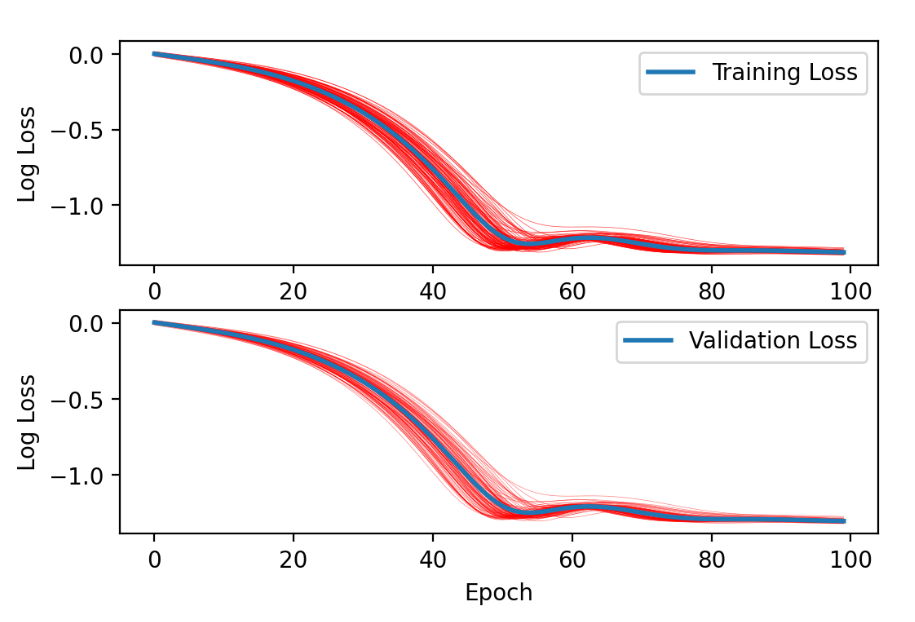
\includegraphics[width=0.8\textwidth]{img/png3.png}
    \caption{Log-loss curves of training and validation losses.}
    \label{fig:space_time_grid}
\end{figure}
\end{frame}

\begin{frame}{Experiment Results}
\begin{figure}[H]
    \centering
    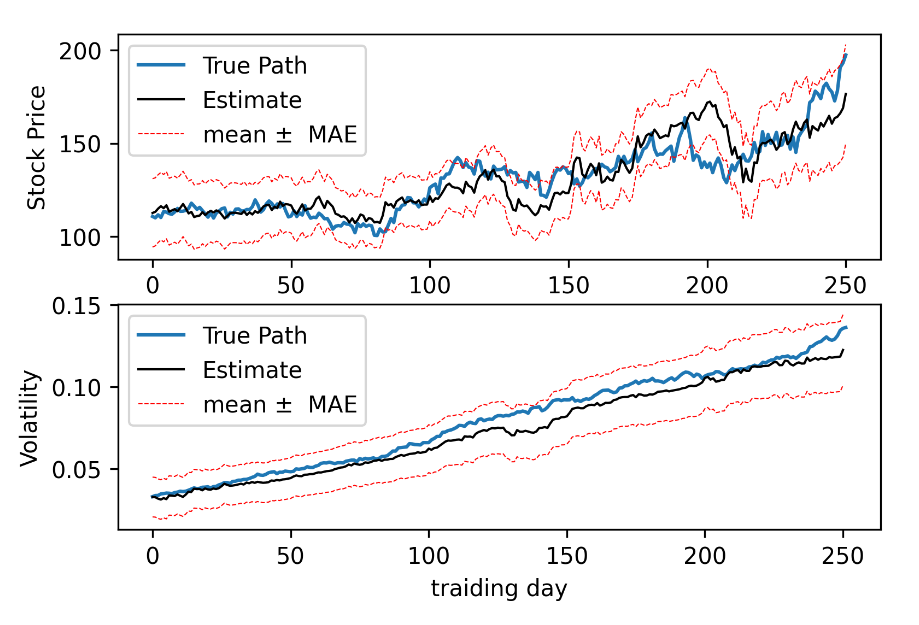
\includegraphics[width=0.6\textwidth]{img/figure2.png}
    \caption{Numerical results of Heston PINN. Top panel: Stock price over a trading year in blue, with the mean PINN prediction in black and the confidence bands at one daily standard deviation. Bottom panel: Volatility of the stock price over a trading year in blue, with the mean PINN prediction in black and the confidence bands at one daily standard deviation.}
    \label{fig:space_time_grid}
\end{figure}

\end{frame}

\begin{frame}{Implication and Limitation}
    1. PINNs train the Heston model adequately.

    2. The estimated mean is largely within one daily standard deviation of the ground truth, indicating that the Heston model is being learned relatively well.

    3. PINNs not only provide accurate predictions but also ensure that these predictions are consistent with known financial rules and structures. 

    4. The experiment conducted with Heston here is not feasible in reality.

\end{frame}

\begin{frame}{Implication and Limitation}
    Is it possible to apply this approach with economic study like macroeconomics?

    Although there is no way we find a parallel universe to test our economic models, we may consider apply this theory on countries of which the characteristics converge (for example, OCED countries).

    Xavier X. Sala-i-Martin. (1996). The Classical Approach to Convergence Analysis. The Economic Journal, 106(437), 1019–1036. https://doi.org/10.2307/2235375
\end{frame}